% Typeset with XeTeX
% Allows use of system fonts rather than just LaTeX's ones
% NOTE - if you use TeXShop and Bibdesk (Mac), can complete citations
%  - open your .bib file, type \citep{xx... and then F5 or Option-Escape
\documentclass[11pt,onecolumn]{article}
\setlength{\columnsep}{6mm}
\usepackage[switch]{lineno} % use option [modulo] for steps of 5
\usepackage[letterpaper,margin=2.5cm]{geometry} % set page layout
%\usepackage{sectsty}
%\sectionfont{\raggedright\large\sffamily\bfseries}
\usepackage[pdftex]{graphicx} % allows us to manipulate graphics.
% Replace option [] with pdftex if you don't use Xe(La)TeX\usepackage{color}
\usepackage{epstopdf} % automatic conversion of eps to pdf 
\usepackage{color} % automatic conversion of eps to pdf 
\usepackage{amsmath, amssymb,bm} % Better maths support & more symbols
%\usepackage{textcomp} % provide lots of new symbols - see textcomp.pdf
% line spacing: \doublespacing, \onehalfspacing, \singlespacing
\usepackage{setspace}
\onehalfspacing
% allows text flowing around figs
% use \begin{wrapfigure}{x}{width} where x = r(ight) or l(eft)
\usepackage{wrapfig}
\usepackage[parfill]{parskip} % don't indent new paragraphs
\usepackage{flafter}  % Don't place figs & tables before their definition 
\usepackage{verbatim} % allows \begin and \end{comment} regions
\usepackage{booktabs} % makes tables look good
\usepackage{bm}  % Define \bm{} to use bold math fonts
% linenumbers in L margin, start & end with \linenumbers \nolinenumbers,
\usepackage[auth-sc]{authblk} % authors & institutions - see authblk.pdf
\renewcommand\Authands{ and } % separates the last 2 authors in the list
% control how captions look; here, use small font and indent both margins by 20pt
\usepackage[small]{caption} 
\setlength{\captionmargin}{20pt}

% ------------------------------------------------------------------------------
%:FONTS
% Using new fonts embedded within the TeX distribution (since 2014)
% For usage, see 'Recent TeX fonts' under the Help menu in TeXShop
% or http://math.ucsd.edu/~msharpe/RecentTexFonts.pdf
% this is also nicer than using System Fonts with XeLatex as it also gets
% math and sans serif fonts correct

%: Bembo-like
%\usepackage[full]{textcomp} % to get the right copyright, etc.
%     \usepackage{fbb} % osf for text, lining for math
%     \usepackage[scaled=.95]{cabin}
%     \usepackage[varqu,varl]{inconsolata}% typewriter
%     \usepackage[libertine,bigdelims,vvarbb]{newtxmath}
%     \usepackage[cal=boondoxo]{mathalfa}% less slanted than STIX
%     \usepackage[T1]{fontenc}
%\useosf

% Libertine
\usepackage{textcomp}
     \usepackage[sb]{libertine}
     \usepackage[varqu,varl]{inconsolata}% sans serif typewriter
     \usepackage[libertine,bigdelims,vvarbb]{newtxmath} % bb from STIX
     \usepackage[cal=boondoxo]{mathalfa} % mathcal
     \useosf % osf for text, not math
\usepackage[supstfm=libertinesups,%
       supscaled=1.2,%
       raised=-.13em]{superiors}
       
       


%:CITATION STYLE
% natbib package: square,curly, angle(brackets)
% colon (default), comma (to separate multiple citations)
% authoryear (default),numbers (citations style)
% super (for superscripted numerical citations, as in Nature)
% sort (orders multiple cites into order of appearance in ref list, or year of pub if authoryear)
% sort&compress: as sort, + multiple citations compressed (as 3-6, 15)
\usepackage[numbers,super,sort&compress]{natbib}

%:NUMBERING STYLE FOR BIBLIOGRAPHY
% (e.g, here it will be 1. and not [1] as in standard LaTeX)
\makeatletter
\renewcommand\@biblabel[1]{#1.}
\makeatother


\usepackage{nicefrac}
\usepackage{multirow}



%:SHORTCUT COMMANDS
% Maths
\newcommand{\ddt}[1]{\ensuremath{\frac{{\rm d}#1}{{\rm d}t}}}  % d/dt
\newcommand{\dd}[2]{\ensuremath{\frac{{\rm d}#1}{{\rm d}#2}}} % dy by dx  - \dd{y}{x}
\newcommand{\ddsq}[2]{\ensuremath{\frac{{\rm d}^2#1}{{\rm d}#2^2}}} % second deriv
\newcommand{\pp}[2]{\ensuremath{\frac{\partial #1}{\partial #2}}} % partial \pp{y}{x}
\newcommand{\ppsq}[2]{\ensuremath{\frac{\partial^2 #1}{\partial {#2}^2}}}
\newcommand{\superscript}[1]{\ensuremath{^{\textrm{#1}}}} %normal (non-math) font for super/subscripts in text
\newcommand{\subscript}[1]{\ensuremath{_{\textrm{#1}}}}
\newcommand{\positive}{\ensuremath{^+}}
\newcommand{\negative}{\ensuremath{^-}}
% Editing
\newcommand{\red}[1]{{\color{red}{#1}}}
\newcommand{\redtext}[1]{{\color{red}{#1}}}
\newcommand{\blue}[1]{{\color{blue}{#1}}}
\newcommand{\bluetext}[1]{{\color{blue}{#1}}}
\newcommand{\scinot}[2]{\ensuremath{#1 \times 10^{#2}}}
% Standard stuff
\newcommand{\be}{\begin{equation}}
\newcommand{\ee}{\end{equation}}
\newcommand{\bea}{\begin{eqnarray}}
\newcommand{\eea}{\end{eqnarray}}
\newcommand{\ie}{\textit{i.e.}}
\newcommand{\etal}{\textit{et al.}}
\newcommand{\khi}{Ki67$^\text{hi}$}
\newcommand{\klo}{Ki67$^\text{lo}$}
\newcommand{\looic}{\ensuremath{\Delta \text{LOO-IC}}}

% \begin{graybox} text \end{graybox} for text with a background colour
\definecolor{MyGray}{rgb}{0.96,0.97,0.98}
\definecolor{MyGray}{rgb}{0.96,0.90,0.98}
\makeatletter\newenvironment{graybox}{%
   \begin{lrbox}
   {\@tempboxa}\begin{minipage}[r]{0.98\columnwidth}}{\end{minipage}\end{lrbox}%
   \colorbox{MyGray}{\usebox{\@tempboxa}}
}\makeatother

%:Title, authors and institutions
\title{Complete and repeated replenishment of the follicular B cell compartment \red{ GC too!} ensures repertoire diversity throughout life}
\author[1]{Melissa Verheijen}
\author[2]{Sanket Rane}
\author[1]{Andrew J. Yates}
\author[1]{Benedict Seddon}
\affil[1]{\small  Institute of Immunity and Transplantation, Division of Infection and Immunity, UCL,  Royal Free Hospital, Rowland Hill Street, London NW3 2PF, United Kingdom}
\affil[2]{Department of Pathology and Cell Biology,  Columbia University Medical Center, 701 West 168th Street, New York, NY 10032, USA}
\date{{\small Address correspondence to either author; {\footnotesize \tt benedict.seddon@ucl.ac.uk, andrew.yates@columbia.edu}}\\
{\small Running title: Complete turnover of naive B cells}\\
{\small Keywords: B cells, mathematical modelling}}
%%%%%%%%%%%%%%%%%%%%%%%%%%
\begin{document}
\maketitle

\linenumbers
%\subsubsection*{Summary}
%Generating and maintaining a diverse repertoire of naive T cells is essential for protection against pathogens, and developing a mechanistic and quantitative description of the processes involved lies at the heart of our understanding of vertebrate immunity. Here we review the biology of naive T cells from birth to maturity and outline how the integration of mathematical models and experiments has helped us to develop a fuller picture of their life-histories.

\section*{Introduction}
B cells v important etc. Develop in bone marrow, where Bcr genes undergo rearrangement. Cells that successfully express a mature BCR migrate to the spleen where they enter a transitional pool of cell, characterised by CD93 expression, and complete development (ref). New B cells enter the spleen and first upregulate CD23 followed by downregulation of IgM. These markers together identify three stages of transitional cell maturation. During the T1 stage, B cells with autoreactive BCRs undergo negative selection. During the T2 stage, cells commit to either a follicular B cell fate, progressing through the T3 stage or are diverted to develop into marginal zone B cells, losing expression of CD23, upregulating IgM and expressing CD21.
Survival of mature B cells is dependent upon BAFFR and BCR signalling. Blockade of BAFF in vivo results in a rapid loss of mature B cells, while BAFFR-/- mice undergo normal BM development and generation of transitional populations, but fail to accumulate mature follicular or marginal Z B cells. Similarly, signals from the BCR are critical for B cell survival. Ablation of BCR expression by  mature B cells results in their rapid loss~\citep{Lam:1997ve}. Expression of Syk, that transmits signals from the BCR, is also required for long term survival of both follicular and MZ B cells~\citep{Schweighoffer:2013jx,Konigsberger:2015gl}.

While it is clear that establishment of the B cell pool relies upon \textit{de novo} generation of B cells in the bone marrow, it is less clear how the stable B cell compartment is maintained in the steady state through out life. B cells have been reported to undergo homeostatic proliferation in lymphopenia~\citep{MeyerBahlburg:2008bc, Cabatingan:2002fm} and there is also evidence of quorom sensing in controlling the overall size of the B cell compartment (Freitas refs). However, it is not known what the relative contribution of self renewal and bone marrow development play in maintaining the compartment. Much of our understanding B cell homeostasis in the steady state comes from analysing BrDu DNA label incorporation. Developing B cells undergo extensive expansion as pre-B cells prior to BCR rearrangement, but remain quiescent and non cycling thereafter  as they develop through transitional stages~\citep{Srivastava:2005jja}. Thus, monitoring the kinetics with which new BrdU labelled cells emerge and are incorporated into the mature pool provides information about B cell life spans and pool maintenance. Such studies reveal that the bone marrow does make substantial daily contribution to the mature follicular pool, estimated at \scinot{3.8}{5} cells a day. Early studies suggest that turnover in B cells in adult mice is slow, with only around half the pool replenished over a 12 week period, and that labelled cells incorporate in a non-linear manner, reaching a plateau over this time period~\citep{Forster:1990tl, Fulcher:1997dr}. 

Blocking B cell development by interfering with IL-7 signalling suggests that mature B cells can persist for weeks to months~\citep{Grabstein:1993jb}. Similarly, inducible deletion of Rag2 results in loss of B cell production, and similar estimates of B cell life span, with 90\% of cells lost within 4 months~\citep{comp:2001ti}. Resource competition is thought to limit the overall size of the B cell compartment. The numbers of B cells found in parabiosed WT pairs vs Rag2\superscript{-/-} and WT mice is the same, despite the latter mice having half the output of new B cells from the bone marrow~\citep{Agenes:1997hk}. There is also the view that the peripheral B cell pool is heterogeneous \red{isn't this unsurprising since there are multiple subsets?}, containing both short lived and long lived populations, although this likely reflected immature and mature populations~\citep{Fulcher:1997dr}.

Despite this extent of study, we still lack understanding of how B cell compartments are maintained throughout the life course. BrdU labelling studies are necessarily limited in duration, due to analogue toxicity in the longer term. Similarly, use of irradiated chimeras to monitor dynamics of repopulation and maintenance are complicated by the lymphopenic environment that induces transitional cells to undergo homeostatic proliferation~\citep{MeyerBahlburg:2008bc}. To address these issues, we employed the method of temporal fate mapping (hogan cite) to measure the contribution and extent of tonic reconstitutions of B cell compartments from the bone marrow. We then tested different models of B cell maintenance to find the most parsimonious explanation for the dynamics during life. 

\clearpage
\section*{Results}
\subsection*{Busulfan treatment permits reconstitution of bone marrow HSC niche without perturbing peripheral mature B cell compartments}
%figure 1 model validation
In order to determine the rules governing the maintenance of peripheral follicular mature (FM) B cell pools, and assess the contribution of de novo B cell development to this , we analysed B cell compartments using a previously published method of temporal fate mapping~\citep{Hogan:2015bd}. Briefly, in this approach, treatment of mice with the conditioning drug, busulfan, ablates the host haematopoetic stem cell (HSC) compartment but leaves mature peripheral haematopoetic compartments unaffected. The depleted HSC niche is then specifically reconstituted with congenically labelled HSC progenitors. Although host HSC replacement is rarely complete, levels of 80-95\% replacement with donor  HSC are typical, and measuring the emergence of donor derived cells serves as an accurate proxy for new cell development from the time of BMT. \red{Do we need to say this? it makes us look more approximate than we are... as long as we normalise to the BM or transitionals, it doesn't matter what chimerism we achieve!} ''The infiltration and replacement of mature peripheral haematopoetic compartments by the progeny of donor HSC can then be followed for the remainder of the hosts life (Figure~\ref{fig:Model_validation}A ). 
%fig 1A - busulfan model

To analyse the maintenance of FM B cells by temporal fate mapping, we generated chimeras by treatment of CD45.1 C57Bl6/J hosts with busulfan followed by their reconstitution with T and B depleted bone marrow from CD45.2 C57Bl6/J donors. We have previously confirmed that busulfan treatment has no detectable impact upon the long-term survival, proliferation nor maintenance of peripheral T cell compartments~\citep{Gossel:2017iu,Hogan:2015bd}. However, to confirm that the same was also true for mature B cell compartments, we compared absolute numbers and expression of Ki67 amongst peripheral B cells at different times following busulfan treatment  and  reconstitution.  As compared with untreated, age matched controls, we observed no significant effects upon either cell numbers or Ki67 levels amongst either transitional, FM or GC B cells (Figure~\ref{fig:Model_validation}B).
%fig 1B - scatters of cell no. vs age in chimeras vs WT in T1, MZ, FM and GC populations - and perhaps a summery of Ki67 too ? 

In order to use emergence of donor B cells as a proxy for total new B cell development since BMT, 
%\red{again, I don't think this is what we are doing. We never need to say that all new cells are donor-derived. it's just that the donor cells are a constant proportion of the new cells}  
knowledge of donor/host chimerism in HSC or B cell progenitor pools is required. Measuring chimerism in B cell progenitors of bone marrow from different bones revealed subtle variations between sites (Fig. S1). Such variations in chimerism were not observed amongst mature B cell populations in individually processed lymph nodes, so did not represent simple technical variation (Fig S1). This most likely reflects variation in the extent of drug mediated HSC ablation, perhaps due to stochastic variation in drug penetrance of different bones. Therefore, chimerism in no single bone marrow site can be representative of total bone marrow output. Although B cell development is initiated in the bone marrow,  developing B cells must migrate to the spleen to continue development as AA4.1\superscript{+} transitional B cells (ref). In particular, AA4.1\superscript{+} IgM\superscript{hi} CD23\superscript{lo} transitional 1 (T1) subset is an obligate, splenic stage, that the vast majority of bone marrow derived B cells  transit.  Therefore, the donor/host composition of T1 cells represents an aggregate of immediate bone marrow output from all the anatomically distinct sites of haematopoesis at any given time. Consistent with this,  donor chimerism in T1 compartment of chimeras revealed a rapid switch from host to donor origin cells following BMT, reaching levels between \red{X and Y\% }(Figure~\ref{fig:Model_validation}C). Importantly, the extent of donor chimerism remained similar in chimeras over time, suggesting that chimerism, once established, was stable, consistent with previous studies~\citep{Hogan:2015bd}. Therefore, we used donor chimerism in T1 compartment as a proxy for de novo B cell development since BMT.
%fig S1 - % donor in different bones
%fig 1C gating for B220 vs AA4.1, LgM vs CD23, donor vs host - then show % donor in T1 vs time post BMT

\subsection*{Temporal fate mapping reveals complete replacement of follicular mature pool by HSC progeny}
%figure 2 
We next analysed donor reconstitution amongst CD23\superscript{hi} transitional 2/3 (T2/3) and FM B cells in chimeras. These populations are recirculating between LN, spleen and bone marrow. Consistent with this, there was a high degree of correlation in donor chimerism observed in these populations at the different lymphoid sites in individual mice. This confirmed that these populations represent a single homogenous pool of mature recirculating cells (Figure~\ref{fig:Raw_FMplots}A). Analysing the changing chimerism with time since BMT revealed rapid replacement of T2/3 cells and progressive replacement of FM B cells (Figure~\ref{fig:Raw_FMplots}B). To visualise the fraction of compartments newly replaced since BMT, we normalised donor fractions in these more mature compartments to the donor fraction observed in T1 splenocytes from the same individual, that is a proxy for the composition of newly generated bone marrow derived B cells. In this way, the fraction of each compartment replaced by new development since BMT can be shown (Figure~\ref{fig:Raw_FMplots}C). As anticipated, T2/3 compartment underwent a complete and rapid replacement within X weeks following BMT. Interestingly, there was a slight delay in the kinetics of replacement of T2/3 cells in LN compared with spleen, that likely reflects the timing involved in differentiation of T1 to T2 and the onset of recirculation and T2 cells populating LN. Strikingly, analysis of the FM compartment underwent a relatively fast and complete replacement in under 20 weeks following BMT.
%2A scatters of % donor in matFM in bm vs spn vs ln
%2B - scatters of raw % donor in T2/3 and FM vs time post BMT
%2C - scatters of FracNew in T2/3 and FM

\subsection*{Ki67 protein levels in developing B cells serve both as a reporter of recent cell division and as a molecular clock}
% Figure 3 - (A) ki67 levels in BM, T1, T2, T3, FM 
% (B) Ki67 frequencies amongst donor and host post BMT
The kinetic of infiltration of donor cells into the FM compartments is rich in information concerning the mechanisms governing the long term maintenance of the pool.
The shifting donor/host composition of FM B cells in chimeras distinguishes cells of different ages, developing either before or after BMT, and is a window into homeostatic mechanisms that may conceal heterogeneity in turnover and/or potentially time-varying rates of loss or proliferative renewal. We also generated chimeras using hosts of varying ages, so that any influence of host age upon B cell maintenance could be discerned. In order to investigate candidate models of B cell maintenance, we analysed data using different mechanistic models of B cell maintenance, to see which could best describe the dynamics of the FM B cell compartment throughout life. An important aspect of  such models is to provide data to help distinguish the contribution of death and proliferation to compartment maintenance,  measuring one or other process. We therefore also measured Ki67 levels in different compartments of chimeras as a marker of recent cell division. In T cells, Ki67 expression is induced at G1 stage of cell cycle, prior to cell division, but persists for more than three days after cell division has ended~\citep{Gossel:2017iu,Hogan:2013id}. 

Analysis of Ki67 expression revealed variation in levels at different stages of B cell development in bone marrow, transitional stages and mature FM B cells (Figure~\ref{fig:Ki67}A). Pre-B cells undergo extensive proliferation during development, and expressed high, unimodel distribution of Ki67 expression. In contrast, transitional populations in the spleen do not undergo cell division as they mature~\citep{Srivastava:2005jja}. However, Ki67 levels were also high in these populations, while only a small subset of FM B cells were found to express Ki67 (Figure~\ref{fig:Ki67}A). Studies of B cell development measuring appearance of BrdU-labelled B cells detect BrdU$^{+}$ T2 cells in the spleen as soon as 2 days after administration of label~\citep{Srivastava:2005jja}, suggesting that the time between cessation of cell division of progenitors in the bone marrow and the development of their progeny can be as little as 2 days, far shorter than the 3-4 day lifetime of Ki67 protein suggested by T cell studies. Therefore, it is most likely that Ki67 expression measured in transitional populations does not represent active cell division, but is rather inherited from  cell division events amongst precursors in the bone marrow. Consistent with this view, Ki67 levels in transitional populations remained unimodal in distribution but exhibited a progressive fall in median level as cells matured through the transitional stages and entered the mature FM compartment (Figure~\ref{fig:Ki67}A). In FM B cells, a smaller subset of cells expressed Ki67. While this may indicate cell division of mature cells, contributing to the maintenance of the pool, some expression also represent residual Ki67 protein present in newly generated B cells. Consistent with such a possibility, analysing Ki67 expression in donor and host cells revealed much higher Ki67 levels amongst donor origin cells, that reduced with time after BMT, to eventually match levels observed in host cells (Figure~\ref{fig:Ki67}B). In light of this, models were formulated in which Ki67 is explained by both the influx of {\khi} progenitors and de novo cell division amongst mature FM B cells. 


\red{2019-02-07 All the FM analysis being redone to accommodate the YFP data - putting constraints on turnover parameters. So blue text is to be updated. GC analysis, however is done! Scroll down...}

\blue{
\subsection*{Dynamics of FM B cell maintenance are best described by a time dependent homogenous model}

The  fraction of new cells $f_\text{new}$ in the FM compartment post BMT stabilises close to 1 by about 120d post-BMT, implying the near-complete replacement of the compartment within that timeframe (Figure~\ref{fig:Raw_FMplots}). Complete replacement suggests that the average rates of loss across host and donor cell populations are always equal.
	Measuring the kinetics of  Ki67 expression revealed that immediately following BMT the donor FM cells are highly enriched for recently divided cells, with around 80\% \khi, but this proportion falls slowly to equalise with that of host cells at around 10\% after approximately 100 days.
	
	%We assumed a mean lifetime of Ki67 post-mitosis of 3.5d, and also assumed that \khi\ and \klo\ cells are lost at equal rates $\delta(t)$. The timecourses of host and donor \khi\ fractions were then generated by simulating the model with its best-fit parameters, beginning at the mean \khi\ fractions observed at 12d post-BMT, pooled across all experimental cohorts. See Methods below for details.}
	
	We modelled this behaviour by assuming that cells differentiate into FM B cells at a rate proportional to size of the source population, and all FM cells, whether host or donor, are lost through death or differentiation  at rate $\delta$ and renewed through division  at rate $\rho$. For generality we allowed either of these rates to vary with the age of the host. We fitted each model  simultaneously to the timecourses of the total size, normalised donor chimerism and the proportions of {\khi} cells within host and donor compartments of the FM population (Figure~\ref{fig:results_FM}A and B; see Methods for details). We found strongest support for T1 as the source population for FM and the model in which the loss turnover rate $\delta$ changes with host age and the division rate $\rho$ remains constant. Specifically, total numbers of FM B cells are given by
	\be
	\ddt{N_\text{FM}} = \;  \phi(t) + (\rho - \delta_{0}e^{-rt}) N_\text{FM},
	\label{eq:FM_total}
	\ee
	
	where $\phi(t)$ is the daily rate of influx from the source, which changes little with host age but whose timecourse was represented empirically using a (nearly flat) spline \red{NEEDS REF TO A FIGURE}, and time is measured from age 60 days, at which time the loss rate is $\delta_{0}$. \red{could cut this text following but nobody reading this will have any idea what LOOIC is so it needs a bit of explanation somewhere!}We compared the support for different models using the Leave-one-out information criterion (LOOIC \red{citation}), a measure of the ability of a model to describe the data with a penalty for over-fitting (see Methods for details).  The differences in LOOIC values map to our our relative degrees of belief in two models as $\exp( -{ \looic} /2)$. This time-varying turnover model was superior to the simplest model with constant rates of division and turnover ({\looic} = 8; 98\% in favour of the model of time-dependent turnover) and also superior to the alternative with a time-varying division rate ({\looic} = 10; 99.3\%). We estimate that FM B cells divide slowly, on average every 10 months,  and have a mean residence time (lifetime) of 30 days in 8.5 weeks-old mice. This life expectancy doubles on an average every $\sim$15 months.
	We also predict that approximately 3\% of FM B cells are replaced each day by newly differentiated cells from the T1 population. Parameter estimates with confidence intervals are in Table 2.
	
	The expected lifetime of an individual FM B cell is the inverse of the turnover rate $(1/\delta)$. However B cell clones can also persist by proliferative self-renewal. If one defines as $\lambda$ as the net effect of cell division and turnover (i.e., $\delta - \rho$), then the inverse of this net loss rate ($1/\lambda$) is the mean time for a B cell clone to go extinct (for example, if proliferation exactly matches loss, $\lambda=0$ and a clone will persist indefinitely) Because $\lambda$ decreases with time for FM cells, due to the declining turnover rate $\delta$, we infer that in old animals individual FM clones and their progeny  persist longer in follicles than in younger animals.
	%Even with the low levels of proliferation seen in FM cells longer-lived clones are possible because of increase in survival rate of cells and their progeny.
	
	
	
	\subsection*{No evidence for heterogeneity in turnover within FM B cell populations}
	
	The decline we detect in the net loss rate of FM B cells ($\lambda$) with host age %which we infer derives from progressively increased survival within the FM compartment,
	derives from the gradual slowing of the approach to stable chimerism relative to a kinetic predicted by a  model of constant division and turnover. An alternative explanation of this time-varying kinetic is that the FM pool comprises independent sub-populations with different but constant rates of division and turnover, each fed from the T1 source.  In this scenario, less persistent populations (those with a high net loss rate $\lambda$) will be replaced most rapidly after BMT, giving an initial steep upslope in chimerism. There will then follow a slower increase as the more persistent FM subpopulations (with low $\lambda$) are replaced by donor cells relatively slowly.
	
	We fitted a model of kinetic heterogeneity assuming two independent subpopulations, allowing their relative size and their constant turnover rates ($\delta_{1}$ and $\delta_{2}$) and division rates ($\rho_{1}$ and $\rho_{2}$)  to be free parameters. However this model received lower support than the model of FM cells as a single population with turnover slowing with host age ({\looic} = 7, Table \ref{tab:FM-AICs}).   Indeed there was a very weak signature of kinetic heterogeneity;  the estimated rates of turnover and division of the two FM subpopulations were nearly equal  ($\delta_{1}$ = 0.11 (0.01, 0.5), $\delta_{2}$ = 0.08 (0.01, 0.48), $\rho_{1}$ = 0.02 (0.0007, 0.21), $\rho_{2}$ = 0.02 (0.0007, 0.25)). % and close to that of the simplest homogeneous model with $\lambda$ = 0.029 (0.024, 0.033).
	
	We also found no evidence for any host-donor differences in kinetics in the form of a persistent host-derived `incumbent' population that resists displacement by newer cells (Table~1). For a discussion of the incumbent model, see Methods and refs.~\citenum{Hogan:2015bd,Rane:2018if}.
	Another potential mechanism for slowing replacement with host age is a decline in the rate of influx (e.g. a fall in the rate of differentiation from T2) with host age.  We found no evidence for any such decline, modelled as exponential decay \red{Sanket is this what you did?} ({\looic} = 18) and so rejected this possibility.


}


\subsection*{Invasion kinetics of donor-derived GC cells are complete but differ between spleen and lymph nodes}
We next analysed turnover within the  germinal centre (GC) pools in lymph nodes and spleen. GL7\superscript{hi} GC cells are present throughout the mouse lifetime even in the absence of deliberate immunological challenge. The origin and dynamics of these constitutive GC reactions are not well characterised.




\red{Following is all TBC as of 2018-12-17 \\
GC cells are known to derive directly from the mature follicular cells [REF] which circulate freely between spleen and lymph nodes [ref].
Therefore, we used pooled numbers of spleen and LN FM cells as a common source for GL7\superscript{hi} GC B cells.
We found that in both spleen and lymph nodes, the donor chimerism in GC compartment reaches the level of chimerism in the source (FM) population (Figure \ref{fig:results_GC} B), revealing complete replacement of host GC cells by that of donor-derived cells. %\red{We need to be more precise in language. It is not complete replacement by donor cells, since chimerism is not 100\%. It's complete turnover}
%This suggests that the host and donor GC cells follow the same rules of turnover.
Surprisingly, the chimerism in splenic GC cells stabilised twice as fast than their lymph node counterparts ($\sim$120 days for spleen GCs versus $\sim$250 days for LN GCs). 
Due to this  disparity in the invasion kinetics of donor cells between the splenic and LN GC pools, and the presumption that GC cells should not be recirculating, we modeled them separately assuming that recirculating FM cells feed into both these populations with a constant rate over time. 

%\subsection*{B cells participating in GC reactions follow same kinetics of division and loss, irrespective of the age of the host.}
To understand the behaviour of GC B cells we began with the simplest model, where all cells are assumed to divide and turnover with constant rates at all times, thereby implying homogeneity.
This simple homogeneous model provided good visual descriptions of time-courses of cell counts and normalised donor fraction (Figure~\ref{fig:results_GC}) with estimates of mean resident times of 0.6(0.48, 0.8) and 0.8(0.59, 1.1) days for spleen and LN GCs respectively.
The simple model with constant rates of cell-division and turnover also captured the trend in {\khi} fractions in host and donor compartments of splenic and LN GC populations remarkably well ( Figure~\ref{fig:results_GC} ). 
We also found that GC cells divide rapidly, with mean interdivision times of $\sim$0.6 and $\sim$0.8 days for spleen and LN GC cells, respectively.
Because the majority of GC precursors (FMs) have fewer {\khi} cells ($\simeq$ 10\%), we speculate that almost all of the GC cells undergo multiple rounds of division or are lost from the pool rapidly before losing their Ki67 expression, or both.

%This shows that individual B cell clones persist  $\sim$3 times longer in lymph node germinal centres, while in spleen they are lost relatively rapidly (mean clonal lifetime = 42 and 13 days for spleen and LN GCs respectively, Table~\ref{tab:GC-parestm}). 
We estimated that $\sim$0.3\% of  GC in lymph nodes and $\sim$57\% of those in the spleen are replaced every day by new cells seeding from the follicular compartment. \red{These conclusions all subject to change} This difference derives largely from the substantially greater daily influx of cells into splenic GC as a proportion of the respective compartment sizes, because the lifetimes of individual GC reactions, $1/\lambda$, were similar in the two compartments (Table~\red{???}). \red{Andy comment 2018-12-17; Need to be careful.  Percent replacement per day is determined by both $1/\lambda$ (how long each reaction lasts  = clone lifetime) and influx (which gives the number of reactions initiated per day). Let's hold off on conclusions till sanket analysis done }
% are primarily regulated by tissue-specific factors.}  \red {we could mention and show the variable donor fraction between different LN of a given chimeras here maybe - in support of the low input rate  from source in LN}

We further tested whether varying either division or turnover with time improved on the fits provided by the simple homogeneous model. 
Allowing variations in $\rho$ or $\delta$ with host age did not enhance the quality of fits and received poorer statistical support ({\looic}$_{\rho}$ = ? and 5 and {\looic}$_{\delta}$ = 0 and 4.9  for splenic and LN GCs, respectively) as compared to the simple homogeneous model. 
Additionally, the rates of change of $\rho$ or $\delta$ estimated by the time-dependent model were extremely small with confidence intervals spanning across zero, suggesting that the given data can be explained without any changes in division or turnover. % showing large uncertainty in parameter estimates.
Therefore, we speculate that the time-dependent variations in the host environment have little or no effect on the population dynamics of B cells participating in GC reactions.
% $\lambda$ gives the ability of individual clones to persist in the GC follicles.


\subsection*{GC population is maintained by continuous seeding of follicular cells into a kinetically homogeneous population over time.}
The complete replacement that we see in GC cells can also be explained by the presence of kinetically heterogeneous subpopulations that divide and turnover at different but constant rates. 
This model of kinetic heterogeneity assumes that the GC population is comprised of fast and slow subsets (as discussed in FM B cells section).
%The differences in dynamics of these subpopulations result in initial rapid increase in donor fractions followed by slower kinetics that lead to stabilisation to the same levels of donor fractions as seen in the source compartment. 
We found that the kinetic heterogeneity model failed to improve on the fits from simple homogeneous model ({\looic} = 0 and 1.1 for spleen and LN GCs respectively, Table~\ref{tab:GC-AICs}) and produced  strikingly similar estimates of loss rates and division rates for both fast and slow subsets in both spleen and LN GC cells.

We also tested the variant of the kinetic heterogeneity model where the host and donor cells behave differently due to the presence of a persistent incumbent subpopulation in the host compartment.
We assume that this incumbent population is established during neonatal stages as the early waves of self-renewing B cells populate the peripheral compartments that are resistant to displacement by new cells.
The incumbent model returned visually similar fits to the time-course of total counts and normalised donor fractions as that of the simple homogeneous model (not shown).
It also failed to differentiate from the simplest model statistically despite having an extra parameter (Table~\ref{tab:GC-AICs}).
Moreover, the estimates of loss and division rates ($\delta_{\text{INC}}$ and $\rho_{\text{INC}}$) of the incumbent population were nearly equal to the loss and division rates of the displceable subset, showing very weak signature of heterogeneity.
These results favour the possibility that GC populations despite being extremely dynamic are kinetically homogeneous and are sustained by constant feeding from follicular B cells.

%Each instance of GC reaction typically lasts for about 3-4 weeks [Can kesmir and Rob de Boer JI 1999, L. Mesin et al., Immunity 2016].
%During this period individual GC B cells undergo massive expansions and intermittent selection events followed by the rapid collapse of GC clusters. %[Nilushi De Silva and Ulf Klein, Nat. Rev. Imm. 2015, N. Wittenbrink  et al., JI 2010]. 
%This suggests that the majority of GC B cells are short-lived and it is less likely that their turnover or division rates are influenced by the cell-intrinsic changes accumulated over their short stay in germinal centres.
%Therefore, we refrained from using more complex models that allow either the cell-division or turnover of GC B cells to vary with cell-age.
%\red{I have fitted the age-structured model on GC cells and it fails to fit to LN GCs and show $\Delta$ AIC of 380 in spleen GCs.}

Our analysis of FM population dynamics shows that the total size of FM compartment increases with time, due to a gradual decline in their turnover (Figure \ref{fig:results_FM}A, left panel).
We tested whether the rate of influx of FM cells into the GC compartment also varies with host-age, so as to maintain the inflow of constant number of cells over time. 
%The time-dependent changes in the influx rate of FM cells in kinetically homogeneous GC compartment may explain the gradual slow down of donor cell invasion in the GC pool.
We found that allowing the rate of influx to vary with host-age, results in very poor descriptions of the normalised donor fractions in both, spleen and LN GC populations ($\Delta$ LOO-ic of ?? and ?? respectively) and hence rejected this possibility.
\red{Therefore, follicular cells maturing into the GC compartment at any given time are proportional to the size of the FM population at that moment.}



\subsection*{Age associated  B cells linked to host and not cell age}
Our results  indicate that FM and GC cells behave as homogenous compartments. In the case of FM cells, there was evidence that homeostatic compartment was influenced by host age. The idea that age impacts homeostasis of B cell compartments is most evident from studies of age associated B cells (ABCs).  ABCs are a more recently described B cell population that is specifically associated with ageing, as they do not apparent in substantial numbers in mice until after a year of age, after which they accumulate in number. It is not known whether this is a cell intrinsic property of ageing cells or rather influenced by host factors associated with age. To explore this, we analysed the 


}

-----------------------------------------





	\section*{Germinal Center B cells}
	
	\subsection*{Invasion kinetics of donor-derived GC cells differ between spleen and lymph nodes.}
	To explain the replacement  kinetics of GC cells in busulfan chimeric mice, we used diverse models that address the heterogeneity in GC compartment and test the effects of host-age on their dynamics (described above in FM section and in Methods).
	All models were fitted simultaneously to an extensive time-course of total counts, donor fractions ($f_{d}$) and the proportions of \khi cells that spans over a year.
	The donor fractions in Spleen and LN GC compartments were normalised to the donor fractions in the common progenitor population,  T1 cells, so as to compare them across animals with different levels of bone marrow chimerism.
	This also allows us to explore the suitability of splenic T1 and the pools of T2 and FM cells that circulate freely between spleen and LN as the putative source populations for spleen and LN GC cells. 
	
	Our data shows that the normalised $f_{d}$ in splenic GC cells stabilises twice as fast as their lymph node counterparts ($\sim$110 and $\sim$260 days post BMT for spleen and LN GCs, respectively), suggesting a strong disparity in the invasion kinetics of donor cells between these two pools. 
	Additionally, we found that recently divided YFP-tagged splenic GC cells were lost twice as fast as LN GC cells in Ki67-CreER-YFP reporter mice (half life 11 vs 20 days respectively, details in the Methods?).
	Due to such differences observed in the population dynamics of spleen and LN GC cells, we decided to model them separately.
	We assumed a constant rate of source influx in both spleen and LN GC pools and allowed our models to be strongly informed by the rate of turnover ($\lambda$) observed in Ki67-CreER-YFP reporter mice.
	
	
	%: Table 1
	\begin{table}[h!]
		\begin{center}
			\renewcommand{\arraystretch}{1.25}
			\begin{tabular}{l l c c c c} 
				\toprule 
				&         & \multicolumn{4}{c}{\textbf{Model and {\looic}}} \\
				\cline{3-6}
				\textbf{Population} & Source     & {\small Simple homogeneous}&  {\small Time-dependent}    & {\small Kinetic heterogeneity} & {\small Incumbent} \\ 
				\toprule
				SPGC &   T1    &   17           &          9            &           33         &          12        \\ 
				     &   T2    &   10           &          0            &           33         &          9         \\ 
				     &   FM    &   13           &          8            &           32         &          9         \\ 
				\hline
				LNGC &   T1    &   55           &          41           &           12         &          54        \\ 
				     &   T2    &   50           &          42           &           12         &          51        \\ 
				     &   FM    &   12           &          35           &           0          &          38        \\ 
				\hline
				\toprule 
			\end{tabular}
		\end{center}
		\caption{\small \textbf{Comparison of models describing population dynamics of GC B cells}. Loo-ic values obtained using leave-one-out cross validation method are shown relative to that of the best fitting model. We consider {\looic} values $\ge$6 of statistical significance for model selection.} 
		\label{tab:GC-AICs}
	\end{table} 
	
	\subsection*{The population dynamics of spleen GC cells are influenced by the age of the host.}
	We find that the total numbers of spleen GC cells increase over time but the proportions of \khi cells remain constant and almost identical between donor and host cells (Figure~\ref{fig:results_SPGC}).
	These results suggest that there is either a substantial increase is the size of the source population or a decline in the turnover of spleen GC cells with host-age.  
	As observed earlier, the size of FM subset increases over time, but their chimerism changes more slowly and stabilises much later (at $\sim$210 days post BMT) than in spleen GCs, suggesting that transitional (T1 and/or T2) subsets are more likely candidates for the source population. 
	Indeed, we found that the model of time-varying loss (where the net loss rate $\lambda$ declines with host-age) using T2 as the source of spleen GCs, received strongest statistical support ~(Table~\ref{tab:GC-AICs}) and produced best visual descriptions of the trends in total cell counts, normalised $f_{d}$ and proportions of \khi cells in splenic GC cells (Figure~\ref{fig:results_SPGC}). 
	
	Our analysis shows that rapidly dying spleen GC clones are sustained for about 15 days by equally rapid division rate in 7w old mice (Table~\ref{tab:SPGC-parestm}).
	The ability of B cell clones to persist in splenic GC pool increases as animals get older due to a relative increase in their residence time $(\nicefrac{1}{\delta})$ in spleen, which doubles every $\sim$8 months.
	Models in which the rate of source influx or the inter-division time of GC cells varies with host-age produced poorer fits and received inferior statistical support  ({\looic} $\ge 8$).  
	We also find that the maintenance of spleen GC compartment is mainly dependent on the source influx as a fairly large proportion of GC cells in spleen ($\sim$ 36\% of total counts in 7w old mice) are daily replaced by the cells from the circulatory pool of T2 compartment. 
	%The time-dependent model with T2 as the source has the fairly large probability (Akaike weight 94\%) to predict new information as compared to all the other models and sources explored in this analysis. 
	
% Table 2
\begin{table}[h!]
\begin{center}
		\renewcommand{\arraystretch}{1.25}
		\begin{tabular}{l l }
			\toprule
			\textbf{Parameter}                                & \textbf{Estimates and 95\% CI} \\
			\toprule
			%Akaike weight (\% )                                     & 94                   \\
			Source influx $(\# \text{of cells} \times 10^{-3})$      & 4.7 (3.2, 6.8)       \\
			Mean clonal lifespan `$\tau$' at 7w of host age (days)   & 15 (13, 16)           \\
			Mean resident time at 7w of host age  (days)             & 0.46 (0.34, 0.61)     \\			
			Mean inter-division time (days)                          & 0.48 (0.35, 0.64)     \\
			Time taken for $\tau$ to double(months)                  & 7.9 (4.5, 25)        \\
			Average time of loss of Ki67 expression (days)           & 5.2 (3.8, 6.7)  \\					
			\hline
			\toprule 
		\end{tabular}
	\end{center}
	\caption{\small \textbf{Parameter estimates from the best-fit (Time-dependent) model using T2 compartment as the source population for SP GC B cells.}  Credible intervals were estimated by taking 2.5$^{th}$ and 97.5$^{th}$ percentiles of the posterior probability distribution of the parameter values obtained after fitting model to the data.}
	\label{tab:SPGC-parestm}
\end{table} 
	
\subsection*{Lymph node GC population contains the mixture of transient and persistent clones.}
The GC compartment in lymph nodes shows a modest increase in its size over time with steady and high proportions of \khi cells that are almost identical between host and donor sub-populations (Figure \ref{fig:results_LNGC}C), very similar to what observed in the spleen.
We found that the models with assumptions of homogeneity within the GC compartment failed to capture the trend in total cell numbers and slow stabilisation of the normalised $f_{d}$, even after allowing host-age dependent alterations in their turnover. 
The replacement kinetics of LN GC cells were best explained by the model that assumes kinetically distinct subsets within GC population, as reflected by its visual descriptions of the trends in cell counts, normalised $f_{d}$ and fractions of \khi cells in LN GC compartment (Figure~\ref{fig:results_LNGC}) and superior statistical support (Table~\ref{tab:GC-AICs}). 
Our data also identified FM compartment as the most likely source of LN GCs as compared to T1 and T2 Transitional subsets ({\looic} $\ge$ 12, Table~\ref{tab:GC-AICs}).
%Fits from the kinetic heterogeneity model to the time-course  of using FM compartment as the source population are shown in .

Our analysis reveals that some GC clones are extremely short-lived and are cleared from the lymph nodes within days (average clonal lifespan of $\sim$ 5days, Table~\ref{tab:LNGC-parestm}) while others can persist for as long as 2 months (Table~\ref{tab:LNGC-parestm}).
The presence of pre-existing host-derived `persistent' GC clones  may explain the slow replacement kinetics of GC compartment in lymph nodes.
In a 7 week old mouse, the LN GC compartment is equally divided between `transient' and persistent clones and we speculate that this ratio would skew towards latter in older animals.
The accumulation of persistent clones over time may also explain the gradual increases in the pool size of LN GC cells.
We also find that roughly 25\% LN GC cells are replaced daily by the new cells entering from the pool of FM cells that are freely circulating between spleen and LN.


%: Table 3
\begin{table}[h!]
	\begin{center}
		\renewcommand{\arraystretch}{1.25}
		\begin{tabular}{l l l }
			\toprule
			\multirow{2}{*}\textbf{Parameter}                 & \multicolumn{2}{l}{\textbf{Estimates and 95\% CI}} \\
			                                                  & \small{Transient Subset}  & \small{Persistent Subset} \\
			\toprule
			%Akaike weight                                         &\multicolumn{2}{c}{99} \\         
			Source influx $(\# \text{of cells} \times 10^{-2})$    & 7.0 (0.2, 40)        & 24 (12, 43)  \\
			Mean clonal lifespan (days)                            & 5.0 (1.2, 19)        & 68 (34, 130)  \\
			mean resident time   (days)                            & 0.69 (0.42, 1.3)     & 0.90 (0.46, 1.9)  \\				
			mean inter-division time (days)                        & 0.91 (0.47, 2.0)     & 0.79 (0.46, 1.9)  \\
			Fraction of total population at 7w of host age         & 0.51 (0.17, 0.72)    & 0.49 (0.28, 0.83)    \\	
			Average time of loss of Ki67 expression (days)         & 5.1 (3.7, 6.6)       & 5.1 (3.7, 6.6)      \\	
			\hline
			\toprule 
		\end{tabular}
	\end{center}
	\caption{\small \textbf{Parameter estimates from the best-fit (Kinetic heterogeneity) model using FM compartment as the source population for LN GC B cells.}  Credible intervals were estimated by taking 2.5$^{th}$ and 97.5$^{th}$ percentiles of the posterior probability distribution of the parameter values obtained after fitting model to the data.}
	\label{tab:LNGC-parestm}
\end{table} 
	
	\begin{figure}[h!]
		\centerline{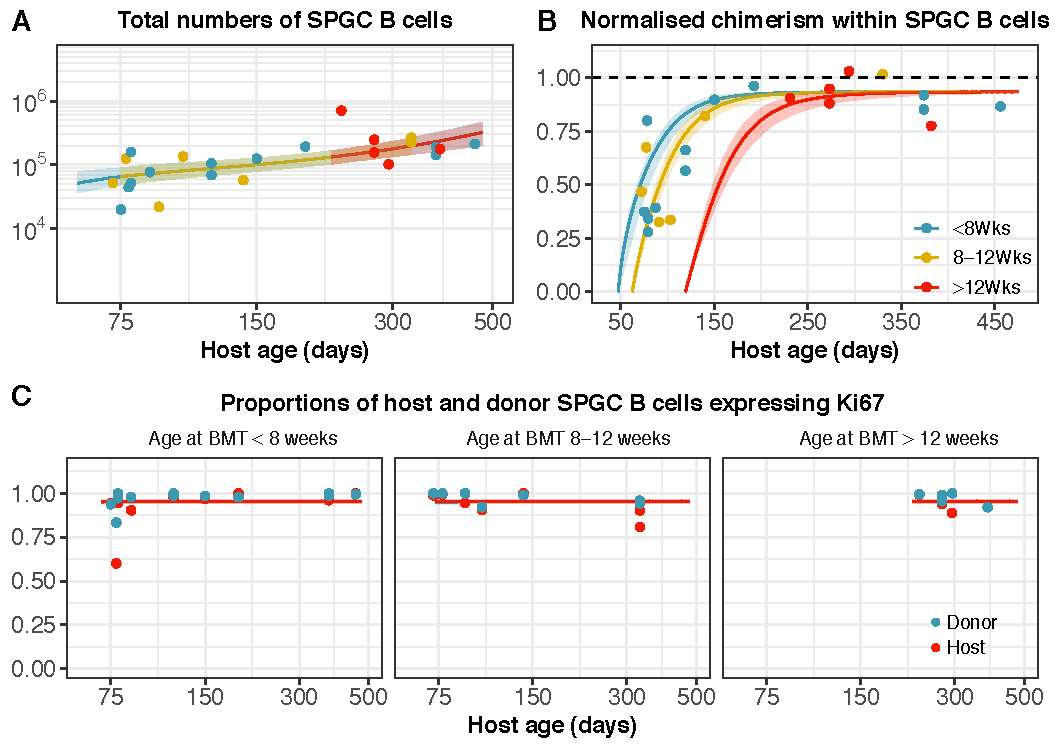
\includegraphics[scale = 0.85] {Results_SPGC_T2.pdf}}
		\caption{\small \textbf{Fitted and predicted population dynamics of spleen GC B cells, using the best-fitting Time-dependent model with T2 as the source.}  The model was fitted simultaneously to the time-course of total cell counts of spleen GC B cells, the donor fractions normalised to the chimerism in T1 cells and the proportions of \khi cells within their host and donor compartments. The time-dependent model fit to the time-course of normalised $f_{d}$ stabilises at a value <1, precisely equal to the ratio of donor fraction in T2 to the donor fraction in T1. Solid lines denote the most probable description of the observations of (A) cell counts, (B) normalised donor fractions and (C) \khi fractions using the time-dependent model with envelopes indicating uncertainty in the model fit. Prediction intervals (4.5$^{th}$ and 95.5$^{th}$ percentiles) were plotted by drawing samples from the posterior distribution of parameter estimates. Different colours in (A) and (B) indicate the different groups of hosts, binned according to the age at which they were transplanted with donor BM cells. Model predictions for individual groups were drawn using the mean age at BMT.}
		\label{fig:results_SPGC}
	\end{figure}
    
    
    \begin{figure}[h!]
    	\centerline{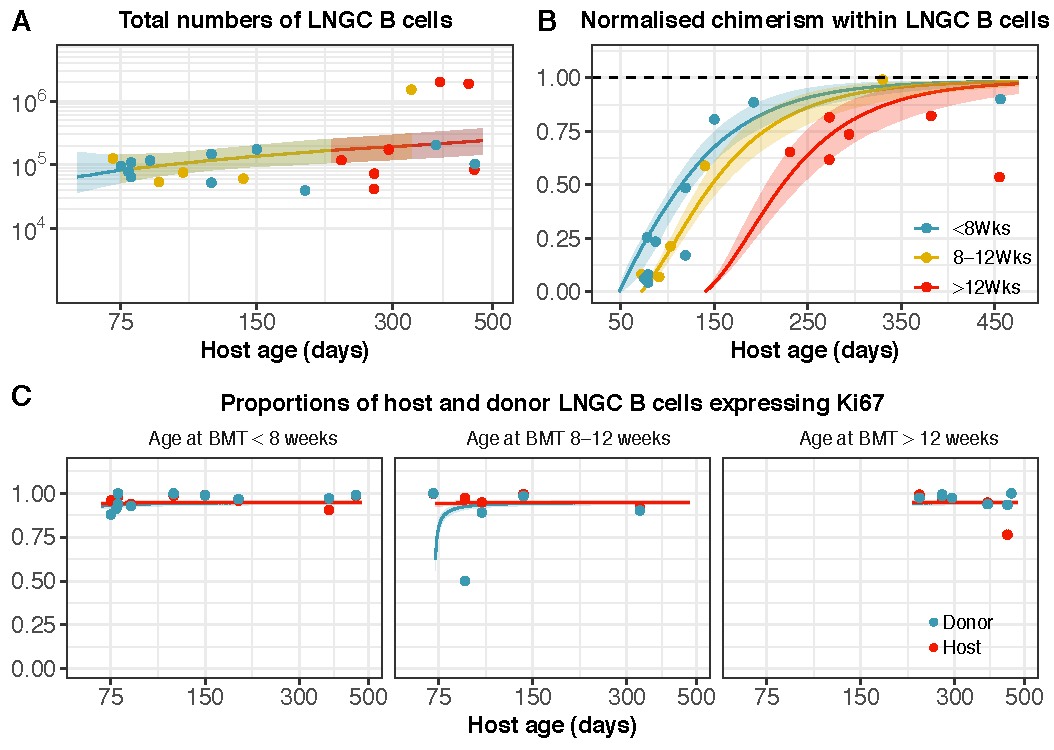
\includegraphics[scale = 0.85] {Results_LNGC_FM.pdf}}
    		\caption{\small \textbf{Fitted and predicted population dynamics of LN GC B cells, using the best-fitting Kinetic heterogeneity model with FM as the source.}  The model was fitted simultaneously to the  time-course of total cell counts of GC B cells pooled from multiple lymph nodes of busulfan chimeric mice, the donor fractions normalised to the chimerism in T1 cells and the proportions of \khi cells within their host and donor compartments.  The kinetic heterogeneity model fit to the time-course of normalised $f_{d}$  approaches 1, following the trend in donor fraction in FM normalised to the donor fraction in T1. Solid lines denote the most probable description of the observations of (A) cell counts, (B) normalised donor fractions and (C) \khi fractions using the time-dependent model with envelopes indicating uncertainty in the model fit. Prediction intervals (4.5$^{th}$ and 95.5$^{th}$ percentiles) were plotted by drawing samples from the posterior distribution of parameter estimates. Different colours in (A) and (B) indicate the different groups of hosts, binned according to the age at which they were transplanted with donor BM cells. Model predictions for individual groups were drawn using the mean age at BMT.}
    		\label{fig:results_LNGC}
    \end{figure}
	




\section*{Discussion}


\section*{Methods}


\section*{Acknowledgements}
The authors acknowledge financial support from the MRC (MR/P011225/1 to BS) and the National Institutes of Health (R01 AI093870 to AY). 



\nolinenumbers % turn off line numbers before references start
% REFERENCES START HERE
% standard bst files are stored in /usr/local/texlive/2007/texmf-dist/bibtex/bst/
% my own are in~/Library/texmf/bibtex/bst/
\bibliographystyle{pnas2009} 

{\small 
\bibliography{rBcell-refs2}
}


\clearpage

%: Table 1
	\begin{table}[h!]
		\begin{center}
			\renewcommand{\arraystretch}{1.25}
			\begin{tabular}{c c c c c} 
				\toprule 
				\multicolumn{4}{c}{\textbf{Model and {\looic}}} \\
				\cline{2-5}
				Source &{\small Time-dependent}  & {\small Simple homogeneous} &  {\small Kinetic heterogeneity} & {\small Incumbent} \\ 
				\toprule
				T1    &   0             &              8             &                7              &          9         \\ 
				T2    &   36            &              43            &                39             &          42        \\ 
				T1 + T2 &   19          &              29            &                28             &          29        \\ 
				\hline
				\toprule 
			\end{tabular}
		\end{center}
		\caption{\small \textbf{Comparison of models describing population dynamics of Follicular Mature (FM) B cells, pooled from LN and spleen}. Loo-ic values obtained using leave-one-out cross validation method are shown relative to that of the best fitting model, in which the rate of loss  (turnover) of FM cells declines slowly with the age of the host. Predictions of more complex models were very close to those of the simple homogenous model (that is, either very little kinetic heterogeneity, close to zero incumbent cells, or effects of cells age on turnover or division rates)}. 
		\label{tab:FM-AICs}
	\end{table} 
	
	\vspace{1cm}
	
	
	%: Table 2
	\begin{table}[h!]
		\begin{center}
			\renewcommand{\arraystretch}{1.25}
			\begin{tabular}{ l r l } 
				\toprule 
				\textbf{Parameter}  &  {\small Estimate}  &  {\small 95\%  $^{\ast}$CI} \\ 
				\toprule
				Total cell numbers at age 8.5 wks ($\times 10^{-6}$)      & 32       &  (24, 43)  \\ 
				Percent daily replacement by source at age 8.5 wks        & 2.7      &  (2.3, 3.0)  \\
				Mean residence time (days) at age 8.5 wks                 & 31       &  (24, 39)  \\ 
				Mean inter-division time (days)                           & 291      &  (129, 2200)  \\
				Time for mean residence time to double (days)             & 470      &  (270, 1400)  \\
				Average time of loss of Ki67 expression (days)            & 6.0      &  (4.6, 7.3)  \\
				\hline
				\toprule 
			\end{tabular}
		\end{center}
		\caption{\small \textbf{Parameter estimates from the best-fit (time-dependent) model for FM B cells (Spleen + LN)}. $^{\ast}$Credible intervals were estimated by taking 2.5$^{th}$ and 97.5$^{th}$ percentiles of the posterior probability distribution of the parameter values obtained after fitting model to the data.}
		\label{tab:FM-parestm}
	\end{table} 


\begin{figure}[htbp] %  figure placement: here, top, bottom, or page
   \centering
%   \includegraphics[width=\linewidth]{Figure.pdf} 
   \caption{(A) Busulfan model cartoon (B) scatters of cell no. vs age in chimeras vs WT in T1, MZ, FM and GC populations - and perhaps a summery of Ki67 too (C) gating for B220 vs AA4.1, LgM vs CD23, donor vs host - then show \% donor in T1 vs time post BMT }
   \label{fig:Model_validation}
\end{figure}


\begin{figure}[htbp] %  figure placement: here, top, bottom, or page
   \centering
%   \includegraphics[width=\linewidth]{Figure.pdf} 
   \caption{(A) scatters of \% donor in matFM in bm vs spn vs ln (B) scatters of raw \% donor in T2/3 and FM vs time post BMT (C) scatters of FracNew in T2/3 and FM }
   \label{fig:Raw_FMplots}
\end{figure}


\begin{figure}[htbp] %  figure placement: here, top, bottom, or page
   \centering
%   \includegraphics[width=\linewidth]{Figure.pdf} 
   \caption{(A) ki67 levels in BM, T1, T2, T3, FM (B) Ki67 frequencies amongst donor and host post BMT }
   \label{fig:Ki67}
\end{figure}


\begin{figure}[h!]
		\centerline{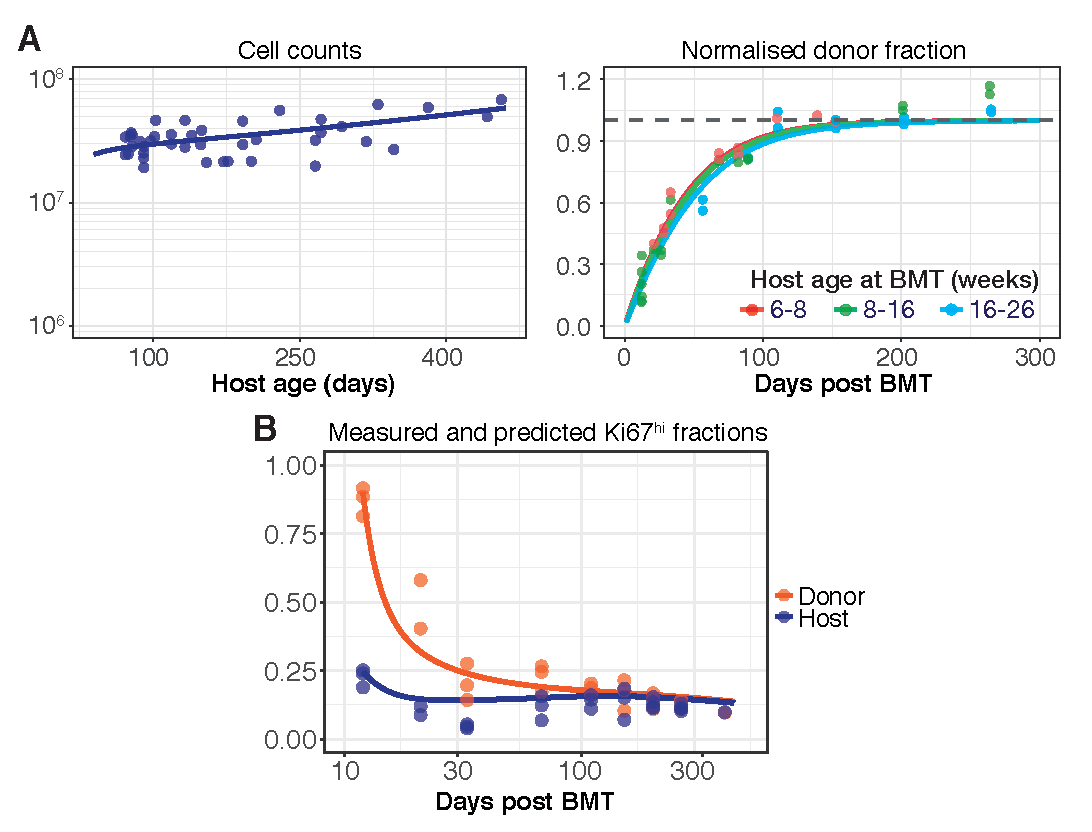
\includegraphics[scale = 0.7] {Results_FM.pdf}}
		\caption{\small \textbf{Fitted and predicted   population dynamics of FM B cells, using the best-fitting model in which cells divide at a constant rate and their mean residence time increases with host age.}  The model was fitted simultaneously to the extended timecourses of total cell counts of FM B cells pooled from LN and spleen in busulfan chimeras, the donor fractions in FM B cells normalised to the chimerism in T1 cells and the proportion of cells that were \khi\ within host and donor FM B cells. Solid lines denote the most probable description of the observations of cell counts and normalised donor fractions and \khi fractions using the time-dependent model with purple envelopes indicating uncertainty in the model fit and the blue envelope indicates uncertainty in the data. Prediction intervals (4.5$^{th}$ and 95.5$^{th}$ percentiles) were plotted by drawing samples from the posterior distribution of parameter estimates.}
		\label{fig:results_FM}
\end{figure}



\begin{figure}[h!]
	\centerline{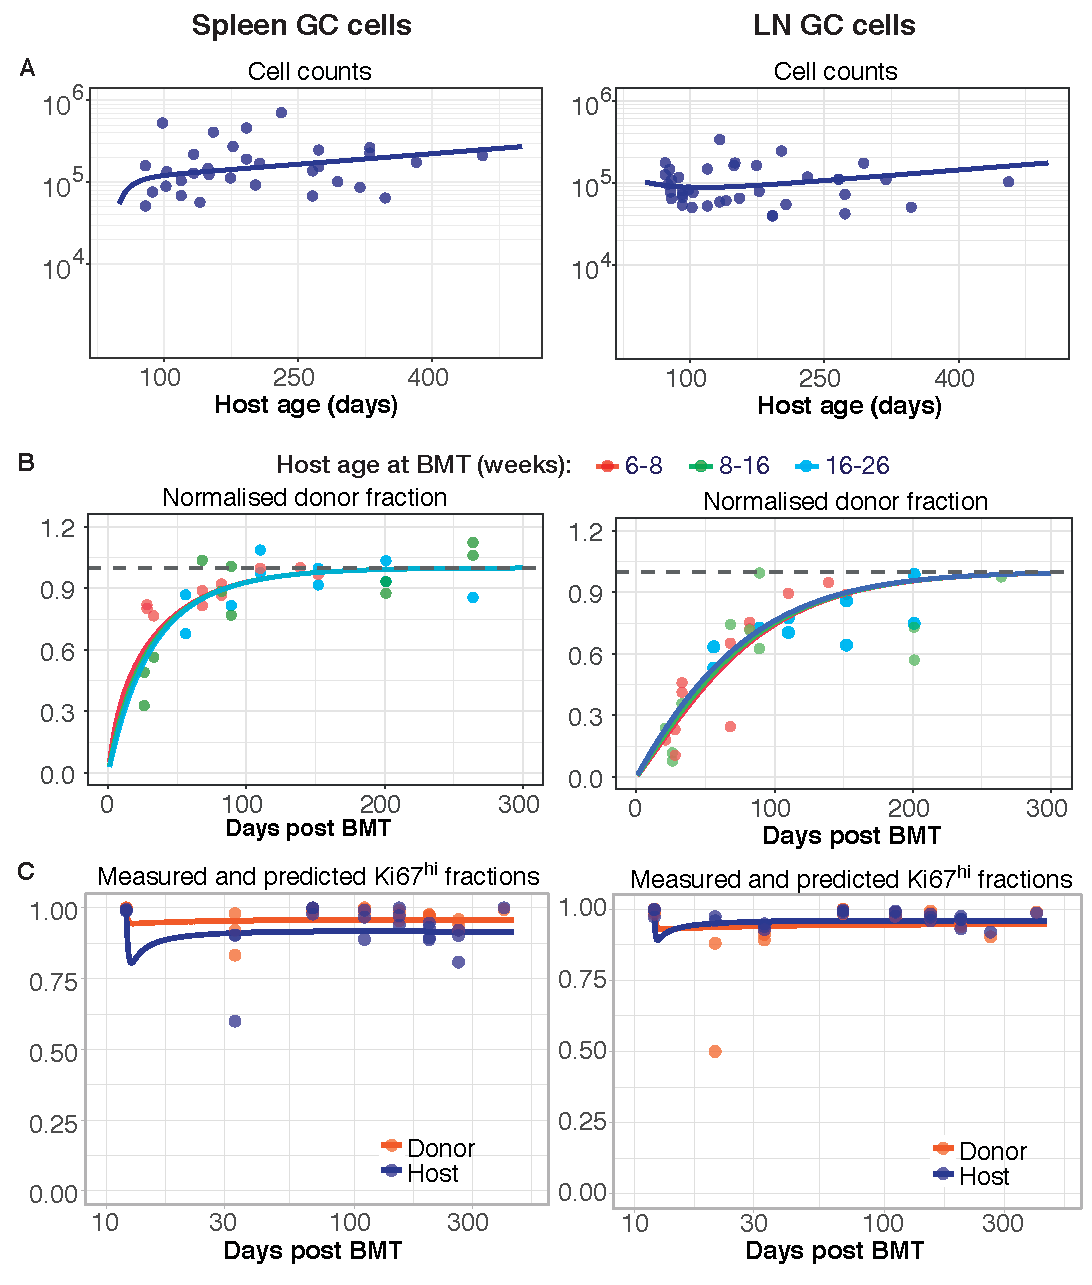
\includegraphics[scale = 0.8] {Results_GC.pdf}}
	\caption{\small \textbf{Fitted and predicted population dynamics of spleen and LN GC B cells, using the best-fitting model in which cells the net loss rate of cells remain constant with time.}  The model was fitted simultaneously to the extended time-courses of total cell counts of spleen and LN GC B cells pooled in busulfan chimeras, the donor fractions normalised to the chimerism in FM B cells and the proportions of \khi cells within their host and donor compartments. Solid lines are the fit from the simple-homogeneous model to the observations (closed circles) of cell counts, normalised donor fractions and the proportion of cells that were \khi\ within host and donor spleen and LN GC B cells, with orange envelopes indicating uncertainty in the model while blue envelope indicate uncertainty in the data. Prediction intervals (4.5$^{th}$ and 95.5$^{th}$ percentiles) were plotted by drawing samples from the posterior distribution of parameter estimates.}
	\label{fig:results_GC}
\end{figure}

%: Table 1
\begin{table}[h!]
	\begin{center}
		\renewcommand{\arraystretch}{1.25}
		\begin{tabular}{ l c c c c} 
			\toprule 
			& \multicolumn{4}{c}{\textbf{Model and {\looic}}} \\
			\cline{2-5}
			\textbf{population}  &  {\small Simple homogeneous}   & {\small Time-dependent} &  {\small Kinetic heterogeneity} & {\small Incumbent}   \\ 
			\toprule
			LN GC cells         & 0   &  4.9  & 1.1 & 2.9   \\ 
			Spleen GC cells     & 0   &  0    & 0   & 1  \\ 			
			\hline
			\toprule 
		\end{tabular}
	\end{center}
	\caption{\small \textbf{Comparison of Loo-ic values obtained using leave-one-out cross validation method are shown for different models fitted to cell counts and donor fractions in spleen and LN GC B cells normalised to the chimerism in FM cells (spleen + LN).}} 
\label{tab:GC-AICs}
\end{table} 

%: Table 2
\begin{table}[h!]
	\begin{center}
		\renewcommand{\arraystretch}{1.25}
		\begin{tabular}{l l r l } 
			\toprule 
			\textbf{Population} & \textbf{Parameter}  &  {\small Estimate}  &  {\small 95\% CI$^{\ast}$} \\ 
			\toprule
			\textbf{Lymph node GC cells} & Total cell numbers at age 8.5 wks ($\times 10^{-3}$)     & 62      &  (23, 188)    \\ 
			& Percent daily replacement by source at age 8.5 wks                                    & 3.3     &  (2.8, 3.5)   \\
			& Mean resident time (days)                                                             & 0.80    &  (0.58, 1.1)  \\ 
			& Mean inter-division time (days)                                                       & 0.80    &  (0.59, 1.1)  \\ 	
			& Average time of loss of Ki67 expression (days)                                        & 5.6     &  (4.2, 7.2)  \\		
			\textbf{Splenic GC cells} & Total cell numbers at age 8.5 wks ($\times 10^{-3}$)        & 7.2     &  (1.8, 30)    \\ 
			& Percent daily replacement by source at age 8.5 wks                                    & 57      &  (38, 97)   \\
			& Mean resident time (days)                                                             & 0.61    &  (0.49, 0.80)  \\ 
			& Mean inter-division time (days)                                                       & 0.60    &  (0.48, 0.79)  \\ 	
			& Average time of loss of Ki67 expression (days)                                        & 6.2     &  (4.9, 7.7)  \\		
			\hline
			\toprule 
		\end{tabular}
	\end{center}
	\caption{\small \textbf{Parameter estimates from the best-fit (simple homogeneous) model for spleen and LN GC B cells.}  $^{\ast}$Credible intervals were estimated by taking 2.5$^{th}$ and 97.5$^{th}$ percentiles of the posterior probability distribution of the parameter values obtained after fitting model to the data.}
	\label{tab:GC-parestm}
\end{table} \


\begin{figure}[htbp] %  figure placement: here, top, bottom, or page
   \centering
   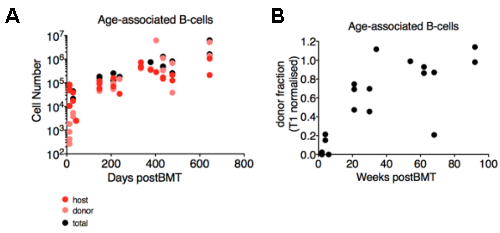
\includegraphics[width=\linewidth]{ABCs.pdf} 
   \caption{(A) Numbers of ABCs in chimeras (B) Donor fraction amongst ABCs normalised to T1 }
   \label{fig:ABCs}
\end{figure}




\end{document}

